\section{Contest results}
\label{sec:results}

We won the contest with a 5--1 record (Table~\ref{tab:rounds}). The competition score is $50P/M + 50$, where $P$ is our points in the Swiss tournament (1 per win) and $M$ is the most points any team received. As the winners we had the most points, so $P = M = 5$ and the score is 100.

\begin{table}[htbp]
  \centering
  \caption{Contest rounds.}
  \label{tab:rounds}
  {\small
  \begin{tabularx}{\textwidth}{@{}c l L L@{}}
    \toprule
    Round & Opponent & Outcome & Why \\
    \midrule
    1 & Team 11 & Won. Our car arrived at the top before team 11. When the cars met, our car pushed back against the force they exerted and got team 11's car on top of ours. Our farthest point was closer, so we won. & The gearmotors got us to the top first, and the forks and wedge plate let team 11's car go over us instead of pushing us off. \\
    2 & Team 08 & Won. Team 08 reached the top first, but went over our car and fell to the end of the ramp, unable to come back. & The forks and wedge plate let the car go over us instead of pushing us off. \\
    3 & Team 09 & Won. We reached the top first and stayed closer to it. The match was close, because both cars ended near the center. & The gearmotors got us to the top first, which gave us the upper hand. \\
    4 & Team 14 & Won. We got to the top first, and because team 14's car was easy for our ramp to get under, we kept our spot under them while they kept driving forward. & The gearmotors got us to the top first, and the low wedge plate slid under team 14's car, so we held our spot while they kept driving forward. \\
    5 & Team 10 & Won. We reached the top later than team 10, but their strategy was to keep going and never stop. Our forks got their car onto ours, and team 10 drove past us and off the ramp. & The forks and wedge plate let the car go over us instead of pushing us off. \\
    6 & Team 05 & Lost. We reached the mesa first and got under the opponent, but stopped short, and its farthest point was closer to the center. & Advance onto the mesa timed, not measured (Section~\ref{sec:lessons}) \\
    \bottomrule
  \end{tabularx}
  }
\end{table}

Our one loss, in the final round, came from the robot's timed advance onto the mesa (Section~\ref{sec:lessons}). We reached the mesa first and got under the opponent, as designed, but the robot stopped short of where it usually did. The opponent's footprint was much smaller than ours, so its farthest point was closer to the mesa center, and we lost on that rule.

\begin{figure}[htbp]
  \centering
  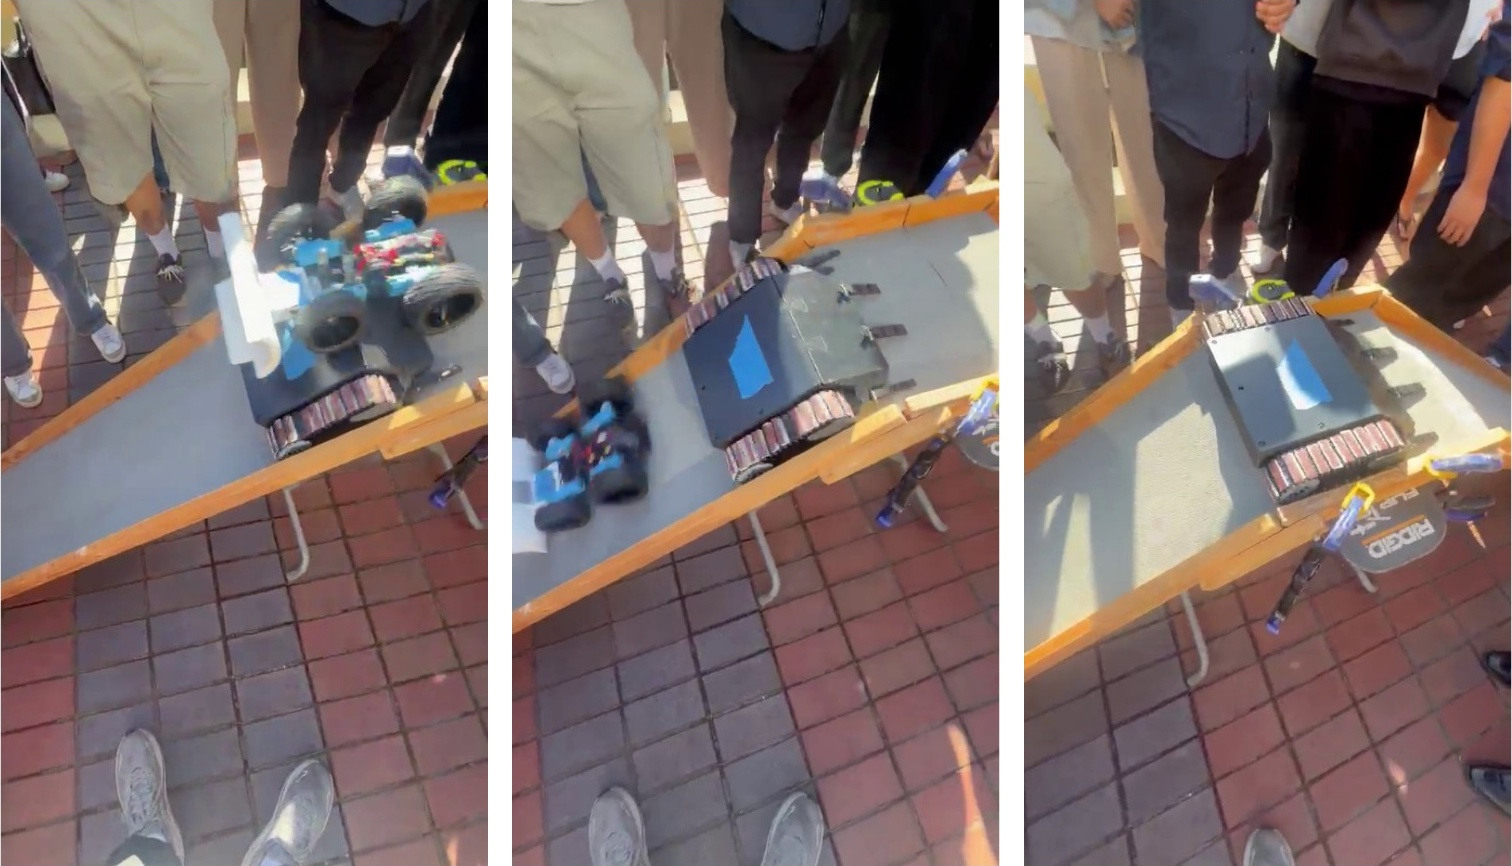
\includegraphics[width=0.9\textwidth]{fig13_contest.jpg}
  \caption{Frames from Round \tbd{N}, left to right. An opponent drives up onto our forks and tips off the side, and our robot holds the mesa alone.}
  \label{fig:contest}
\end{figure}
